\chapter{Measurement of \kzero production in pp collisions}
\label{cap:4}


\vspace*{2cm}
Short lived resonances are good probes to study the properties of strongly interacting matter produced in high energy heavy ion collisions. \kzero~ is a resonance particle with a small lifetime ($\sim$ 4~\fmc), comparable to that of the fireball which is produced during the heavy ion collision. Due to its short lifetime, it can be used to study the re-scattering and regeneration effects. \kzero~ can provide the information regarding strangeness enhancement as it contains a strange quark. Measurements of \kzero~ in pp collisions can be used as a baseline to study the \PbPb~collisions at the LHC energy and to provide a reference for tuning event generators. Study on \kzero was done to learn the analysis procedures. In this way, an already available result could be used as a benchmark to test the method followed in the analysis.


I shall describe the measurement of \kzero~mesons produced at mid-rapidity (\modrap~$\leq$~0.5) in minimum-bias pp collisions at \sqrtS~=~13~TeV. In this analysis, \kzero~ has been reconstructed by its hadronic decay channel $K^{*0} \rightarrow K^{\pm}+ \pi^{\mp}$. The yield of \kzero~is extracted from \pion K~invariant-mass distributions as a function of transverse momentum.  The \pT~spectrum is integrated to obtain a measurement of the total \dndy, and the mean transverse momentum \meanpT~is extracted from the spectrum. 


\section{\kzero reconstruction in pp collisions}
\label{par:4.1}
The \kzero~ production in pp collisions at \sqrtS~= 13 TeV has been done with data collected in 2015 by ALICE detector. The analysis strategy is based on the invariant mass study of reconstructed pairs whose origin could be the decay of \kzero~ mesons into charged particles. The daughter particles are identified as oppositely charged pions and kaons among the tracks reconstructed in the central barrel. Track selection and particle identification is described further in this chapter. To extract the yields of \kzero~ mesons in each \pT~ bin, the invariant-mass distribution of unlike-charge pairs from the same event is computed. The combinatorial background is estimated by event-mixing technique and subtracted from the unlike-charge distribution. In event-mixing technique, the combinatorial background is constructed through the invariant mass of pions and kaons of different events having similar z-vertex, and multiplicity. The mixed event is normalised by the same event distribution in the region of invariant mass of 1.1 to 1.3 \GeVcSq. The signal is obtained by subtracting the mixed event combinatorial background from the same event kaon - pion invariant mass distribution. (see \mbox{Figure \ref{Fig:chap4-4.1}})

\begin{figure}[t]
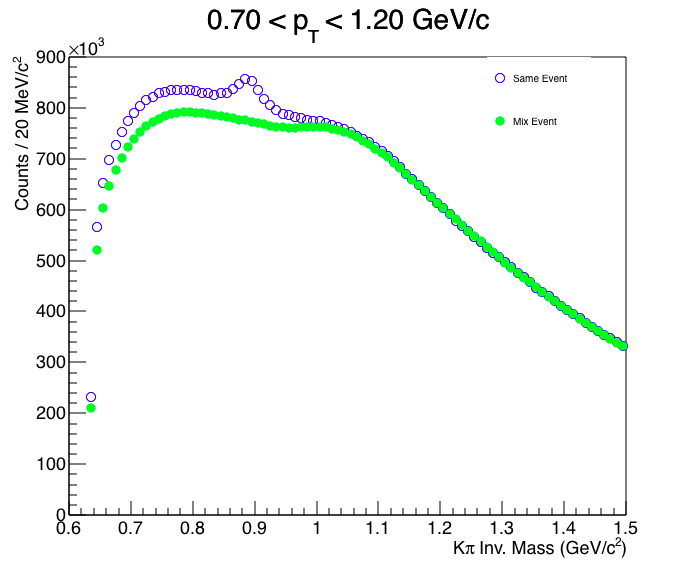
\includegraphics[width=0.45\textwidth]{Images/Chapter4/1mix.png}
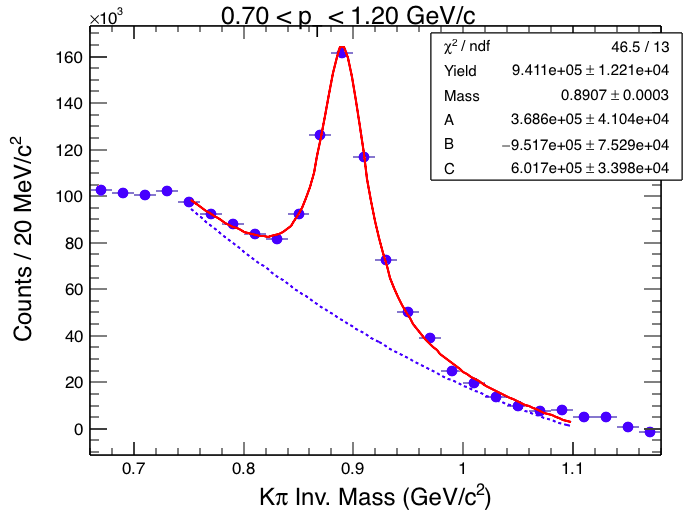
\includegraphics[width=0.48\textwidth]{Images/Chapter4/2sig.png}
\caption{(Left) Unlike-sign invariant mass distribution (open blue circles) and invariant mass obtained by mixed events (green circles) for transverse momentum range $0.7-1.20$ \GeVc. The distribution obtained by event mixing technique is normalised in the range $1.1- 1.3$ \GeVcSq. (Right) Unlike-sign invariant mass distribution after background subtraction for the transverse momentum range $0.7-1.2$ \GeVc. Red curve represents the result of the fit. Blue dashed curve represents the background estimated by a polynomial.}
\label{Fig:chap4-4.1}
\end{figure}

The \pT~ dependent correction due to the detector acceptance and reconstruction efficiency, (\emph{\rm{eff} = \rm{Acc} x $\epsilon_{rec}$})(\pT), is computed using Monte Carlo simulations that describes at relative per cent level the detector geometry and response. $\epsilon_{rec}$ in particular contains the contribution of tracking and candidates selection cuts. Raw counts are also corrected for the decay branching ratio (BR) and final yield is estimated using:

\begin{equation}
\label{Eq:4-4.1}
\frac{d^{2}N}{dp_{T}dy} = \frac{\text{Raw Counts}}{N_{MB} \times BR \times dp_{T} \times dy \times \rm{eff}} \times f_{norm} \times f_{SL}
\end{equation}

where factor $f_{norm}= 0.852^{+0.062}_{-0.03}$ is efficiency for trigger selection for inelastic pp collisions.  The factor $f_{SL} = 0.931264$ accounts for the signal loss introduced by the requirement that a primary vertex must be reconstructed and be in the range of  $\pm 10$ cm.

\section{Data Sample and event selection}
\label{par:4.2}

The data used for this analysis was taken during June 2015 pp run (LHC15f, pass 2 reconstruction \footnote{A few reconstruction processes are needed to obtain data usable for physics analysis. Usually the first two reconstruction passes (pass $0$ and pass $1$) are needed for quality assurance check and calibration of the main detectors. The pass $2$ is the first usable reconstruction for analysis purpose. Further passes are needed to implement signals from detectors requiring special calibrations.}). The full sample consists of 104 runs totalling to about $527 \times 10^{6}$ events. Out of these, only 48 runs have been used, which are marked by the collaboration as 'good runs' i.e. they are characterized by good performance of the detectors and good running conditions (e.g. low level of beam induced background). In particular, all these \virgolette{good runs} have both the TPC and all the ITS sub-detectors turned on.


The purpose of the event selection is to select hadronic interactions with the highest possible efficiency, while rejecting the machine-induced and physical backgrounds. The ALICE on-line minimum bias (MB) trigger for this pp run was configured to require the following two conditions: 

\begin{description}
\item[(i)] a signal above the threshold in V0A,
\item[(ii)] a signal above the threshold in V0C.
\end{description}


The threshold in the VZERO detector corresponds approximately to the energy deposition of a minimum ionizing particle. 


For this analysis, a sample of $45 \times 10^{6}$ minimum bias pp events has been processed where ITS, TPC and TOF performance was optimal. Out of this, around 16 million events satisfy the following selection criteria and have been actually used for the analysis:

\begin{itemize}
\item Is InComplete DAQ check.
\item Pileup Rejection using AliAnalysisUtils::IsPileUpEvent().
\item SPD Clusters vs. Tracklets Check using AliAnalysisUtils::IsSPDClusterVsTrackletBG() with default parameters.
\item Event has a track or SPD primary vertex identified.
\item SPD vertex-z resolution $< 0.25$ cm.
\item SPD vertex dispersion $< 0.04$ cm.
\item z-position difference between track and SPD vertex $< 0.5$ cm.
\item vertex-z position : $|v_{z}| < 10$ cm.
\end{itemize}



\begin{figure}[h!]
\centering
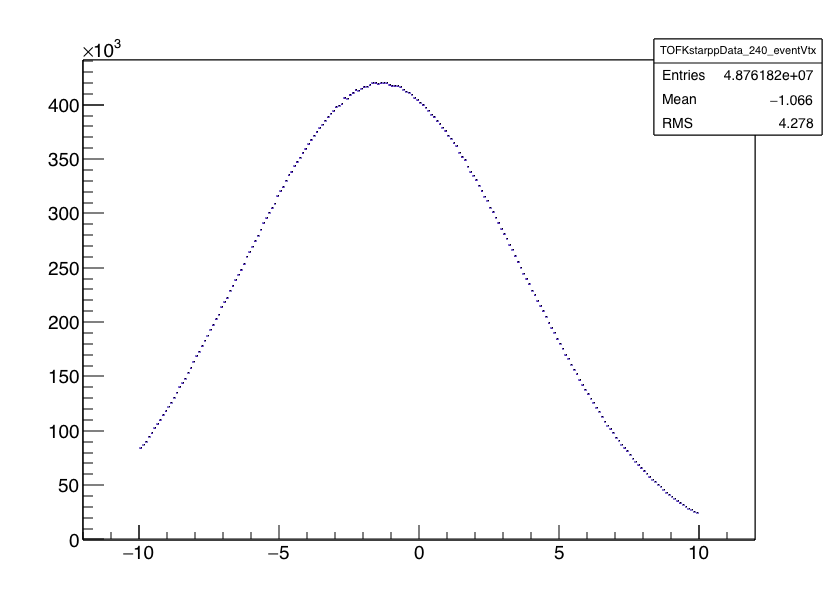
\includegraphics[width=0.7\textwidth]{Images/Chapter4/evt_vtx_k0.png}
\caption{Vertex z coordinate distribution of the accepted events.} 
\label{Fig:chap4-4.2}
\end{figure} 


The distribution of vertex z position of the accepted events is reported in \mbox{Figure \ref{Fig:chap4-4.2}}. Events with $|V_z| < $ 10 cm have been used to ensure a uniform acceptance in the central pseudorapidity region, $|h| < $0.8, where the analysis is performed.

\subsection{Track Selection}
\label{par:4.2a}
The \kzero~ is studied by reconstructing its hadronic decay into charged particles \kcharged $\pi^{\mp}$ (B.R. = 66.6$\%$). Because of its very short lifetime of $\sim 4$\fmc, the resonance decays early after its production and does not make it out of the beampipe. The selection of the candidate daughters is a challenge for the \kzero~ reconstruction, because the produced kaon and pion and undistinguishable from the charged primary particles produced in the \virgolette{bulk}.
The candidate resonance daughters with  $ \pT > $0.15 \gmom~ in the pseudorapidity interval $|h| < 0.8$, are first of all selected by applying cuts on the quality of the reconstruction, related to:

\begin{itemize}
\item Reject kink daughters.
\item Minimum number of rows crossed in TPC is 70.
\item TPC $\chi^{2}$ clusters $<4.0$
\item ITS $\chi^{2}$ clusters $<36.0$
\item $|\text{DCA}|_{z} < 2 $ cm
\item $(\text{DCA})_{r}< 0.0105+ 0.0350p_{T}^{-1.01}$
\item  Pair rapidity $< |0.5|$
\end{itemize}


The cuts listed above define the \virgolette{standard quality cuts}.


\subsection{Particle Identification}
\label{par:4.2b}
The daughter particles of \kzero are charged kaons and pions and they can be identified by using Time Projection Chamber (TPC) and Time Of Flight (TOF) detectors.  Particle identification in TPC is performed by measuring the specific energy loss (\dedx) in the detector gas. The energy loss is described by the Bethe-Bloch function:
\begin{equation}
 \langle{dE\over dx}\rangle = {4\pi N e^{4} \over mc^{2}} {Z^{2} \over \beta^{2}} \Bigl(\ln{2mc^{2}\beta^{2}\gamma^{2} \over I} - \beta^{2} - {\delta(\beta) \over 2} \Bigr) \; ,
 \label{eq.:Bethe}
\end{equation}
\noindent where mc$^{2}$ is the rest energy of the electron, $Z$ the charge of the projectile, $N$ the number density of electrons in the traversed matter, $e$ the elementary charge, $\beta$ the velocity of the projectile and $I$ is the mean excitation energy of the atom. A truncated mean that rejects the $40\%$ largest cluster charges is built, resulting in a Gaussian \dedx~ response. The measured energy loss is compared to standard energy loss (Bethe-Bloch function) for different particles to identify them. The \dedx~ resolution ranges between $5 - 8\%$ depending on the track inclination angle and drift distance, the energy loss itself and the centrality of the collisions due to the different detectors. \\
\\
The TOF detector is based on Multigap Resistive Plate Chamber technology. It measures the time of flight of particles with an intrinsic resolution of $\sim 80 $ ps. The expected flight time for each particle species is calculated during the reconstruction, and then PID is performed via a comparison between the measured and expected times. Both pions and kaons are selected by a cut of $|N\sigma_{\rm{TPC}} | < 2.0$ with a TOF veto of $|N\sigma_{\rm{TOF}} | < 3.0$. TOF veto means that the TOF cut is applied only for cases where the track matches a hit in the TOF. (see \mbox{Figure \ref{Fig:chap4-4.3a}} and \mbox{Figure \ref{Fig:chap4-4.3b}})



\begin{figure}[ht]
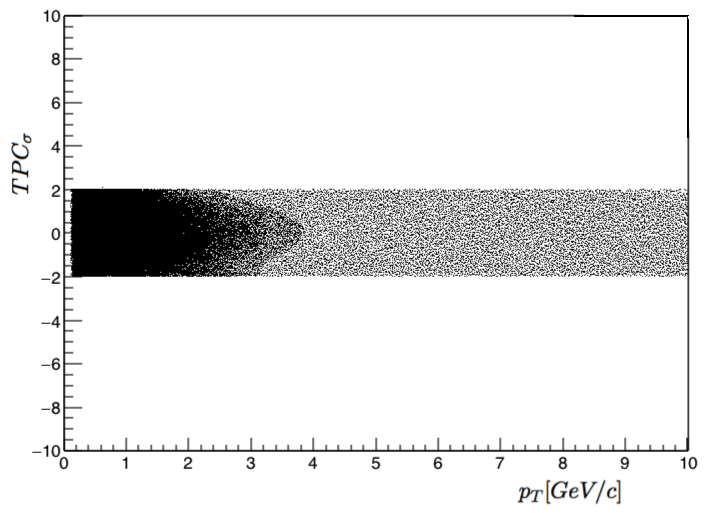
\includegraphics[width=0.49\textwidth]{Images/Chapter4/tpcsigmapi.png}
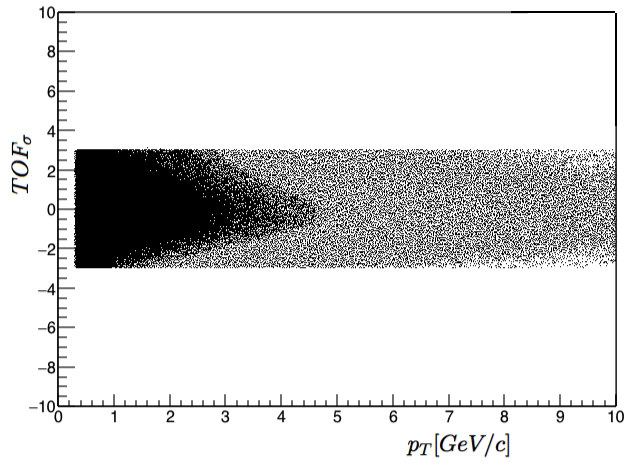
\includegraphics[width=0.49\textwidth]{Images/Chapter4/tofsigmapi.png}
\caption{(Left) TPC sigma for $\pi$ vs $p_{T}$. (Right) TOF sigma for $\pi$ vs $p_{T}$}
\label{Fig:chap4-4.3a}
\end{figure}


\begin{figure}[ht]
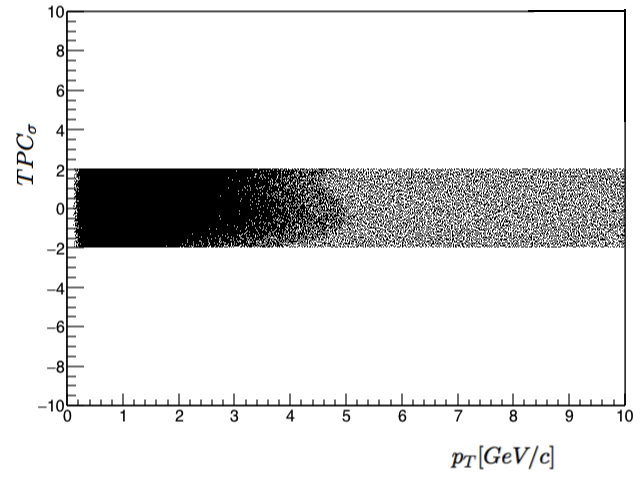
\includegraphics[width=0.49\textwidth]{Images/Chapter4/tpcsigmak.png}
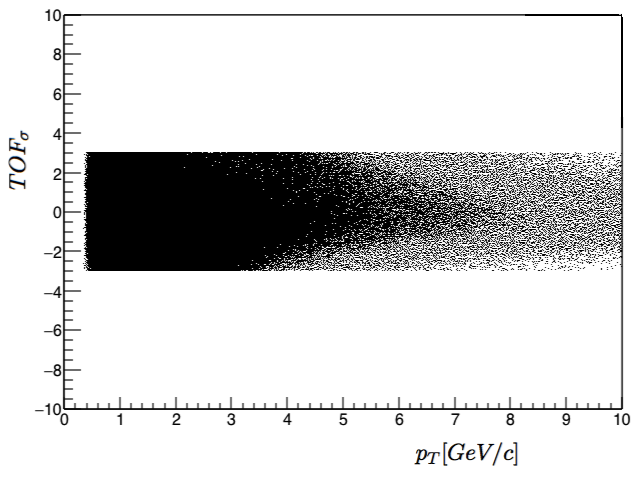
\includegraphics[width=0.49\textwidth]{Images/Chapter4/tofsigmak.png}
\caption{(Left) TPC sigma for $K$ vs $p_{T}$. (Right) TOF sigma for $K$ vs $p_{T}$}
\label{Fig:chap4-4.3b}
\end{figure}

\section{Signal Extraction using Event Mixing}
\label{par:4.3}
To extract the yields of \kzero~ mesons in each \pT~ bin, the following procedure is used. The invariant-mass distribution of unlike-charge pairs from the same event is computed. The combinatorial background is estimated by event-mixing technique and subtracted from the unlike-charge distribution. \\
\\
In event-mixing technique, the combinatorial background is constructed through the invariant mass of pions and kaons of different events having similar z-vertex, and multiplicity. For the reconstruction, we mix 5 events which have z-vertex difference within 1 cm and multiplicity difference within 5. The mixed event is normalised by the same event distribution in the region of invariant mass of 1.1 to 1.3 \GeVcSq. (see \mbox{Figure \ref{Fig:chap4-4.4}})
The signal is obtained by subtracting the mixed event combinatorial background from the same event kaon - pion invariant mass distribution. (see \mbox{Figure \ref{Fig:chap4-4.4}})


After subtraction of combinatorial background, a certain amount of background is left under the \kzero~ signal, which is known as residual background. The source of this residual background may be:
\\
1. correlated real $K\pi$ pairs from other resonance decay.
\\
2. correlated but misidentified $K\pi$ pairs.
\\
 The invariant mass calculated from misidentified pairs can not be subtracted away by mixed event background and it remains as a residual background.





\begin{figure}[ht]
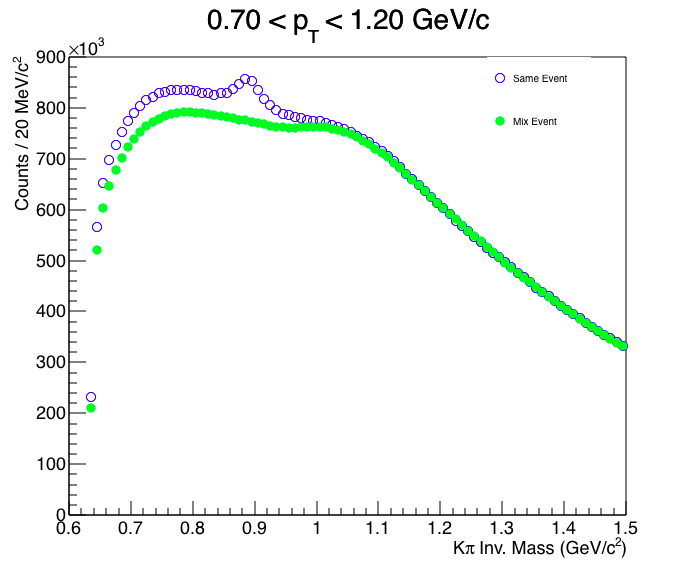
\includegraphics[width=0.45\textwidth]{Images/Chapter4/1mix.png}
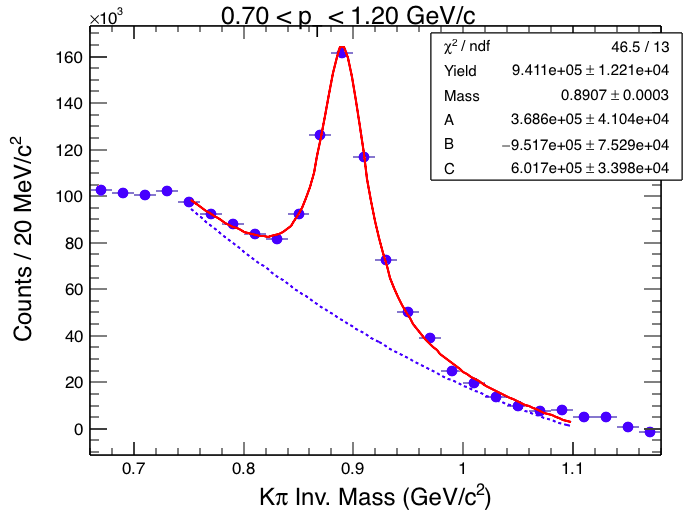
\includegraphics[width=0.48\textwidth]{Images/Chapter4/2sig.png}
\caption{(Left) Unlike-sign invariant mass distribution (open blue circles) and invariant mass obtained by mixed events (green circles) for transverse momentum range $0.7-1.20$ \GeVc. The distribution obtained by event mixing technique is normalised in the range $1.1- 1.3$ \GeVcSq. (Right) Unlike-sign invariant mass distribution after background subtraction for the transverse momentum range $0.7-1.2$ \GeVc. Red curve represents the result of the fit (see text). Blue dashed curve represents the background estimated by a polynomial (see text)}
\label{Fig:chap4-4.4}
\end{figure}




\section{Mass}
\label{par:4.4}
The background-subtracted unlike-charge invariant mass distribution is fitted by a function given by the sum of a non-relativistic Breit-Wigner function and a second order polynomial.
$$\frac{Y}{2\pi}\frac{\Gamma_{0}}{(M_{K\pi} - M_{0})^{2}+  \frac{\Gamma_{0}^{2}}{4}} + Polynomial$$

where $M_{0}$ and $\Gamma_{0}$ are the mass and width of the $K^{*0}$, $M_{K\pi}$ is $K\pi$ invariant mass. The parameter Y gives the Breit-Wigner area. The mass values  obtained for the different \pT~ bin are reported in \mbox{Figure \ref{Fig:chap4-4.5}}. \\
	

\begin{figure}[H]
\begin{center}
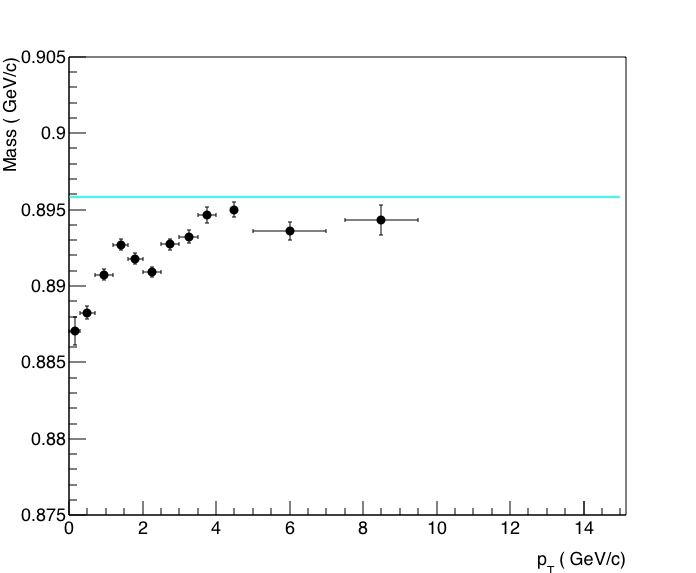
\includegraphics[width= 0.6\textwidth]{Images/Chapter4/mass.png}
\caption{Mass vs. \pT. The line represent the \kstarZ~ PDG mass value.}
\label{Fig:chap4-4.5}
\end{center}
\end{figure}




\section{Raw Yield Extraction}
\label{par:4.5}
\kzero~ raw yield for each \pT~ bin is obtained by fitting the invariant mass distribution while fixing the width value to the PDG one (0.0474 \GeVcSq). The raw yield is obtained from the Y parameters of the Breit-Wigner function. 
\\
The yield has been estimated in 13 \pT~ bins lying between : 0, 0.3, 0.7, 1.2, 1.6, 2.0, 2.5, 3.0, 3.5, 4.0, 5.0, 7.0, 10.0, 15.0 \GeVc. The invariant mass distributions and the fit results for the different $p_T$ bins are shown in \mbox{Figure \ref{Fig:chap4-4.6}}.
\\
\\
The raw yield \pT~ spectrum is shown in \mbox{Figure \ref{Fig:chap4-4.7}}. 

\begin{figure}[h]
\begin{center}$
\begin{array}{cccc}
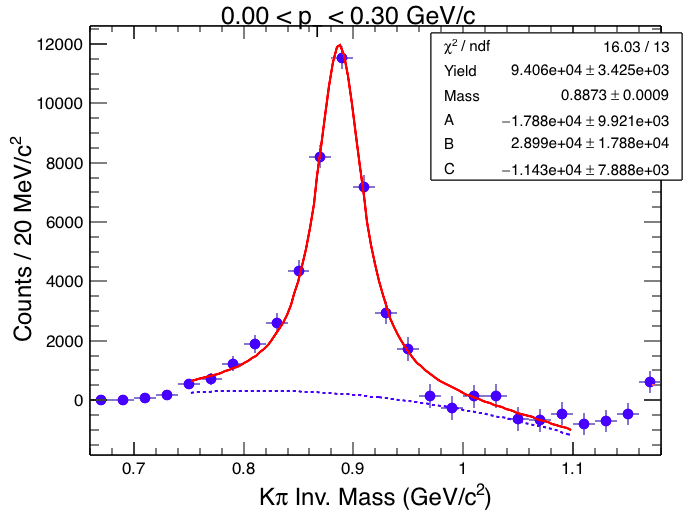
\includegraphics[width=2in]{Images/Chapter4/fit/0.png} &
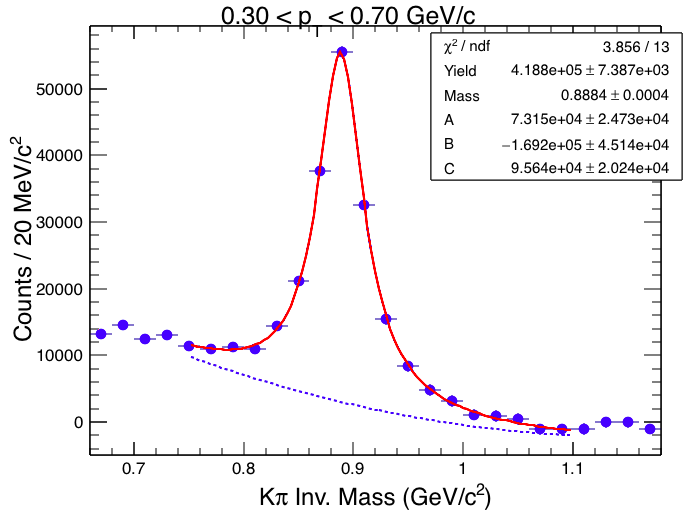
\includegraphics[width=2in]{Images/Chapter4/fit/1.png} &
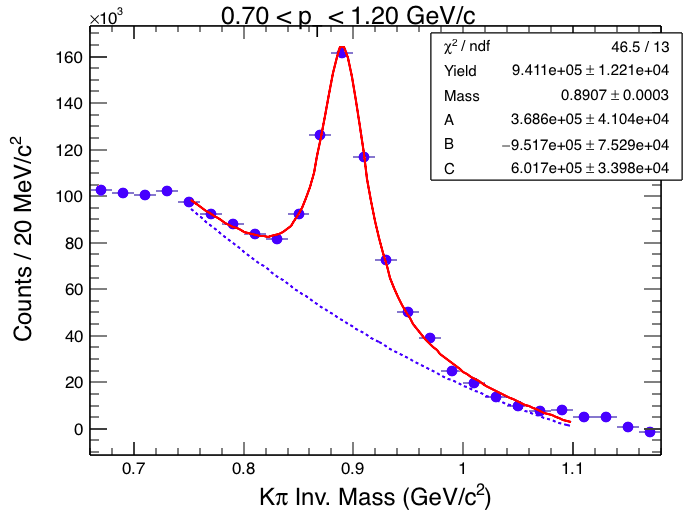
\includegraphics[width=2in]{Images/Chapter4/fit/2.png} \\
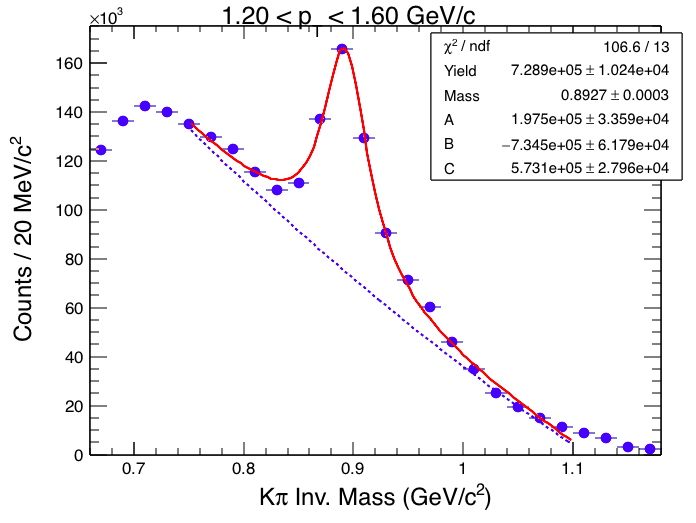
\includegraphics[width=2in]{Images/Chapter4/fit/3.png} & 
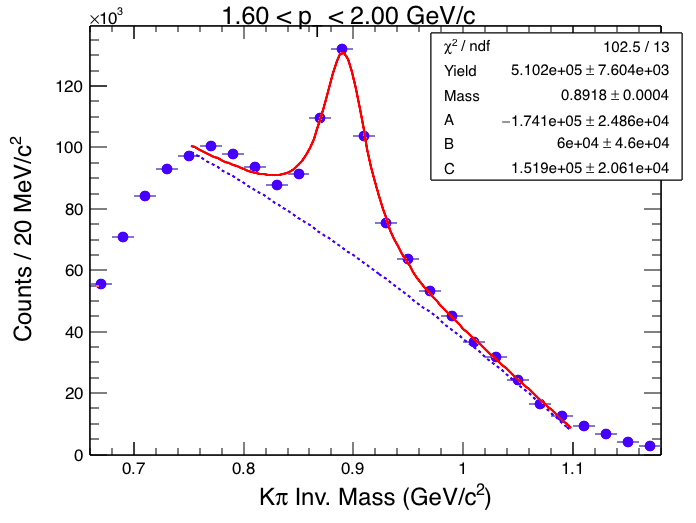
\includegraphics[width=2in]{Images/Chapter4/fit/4.png} &
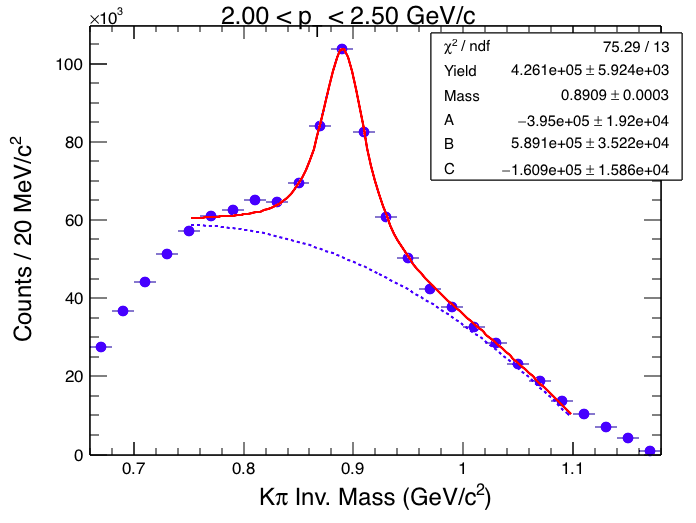
\includegraphics[width=2in]{Images/Chapter4/fit/5.png} \\
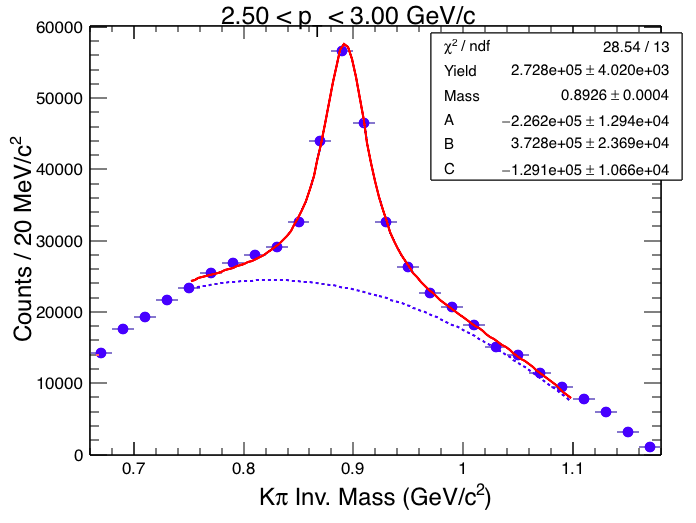
\includegraphics[width=2in]{Images/Chapter4/fit/6.png} &
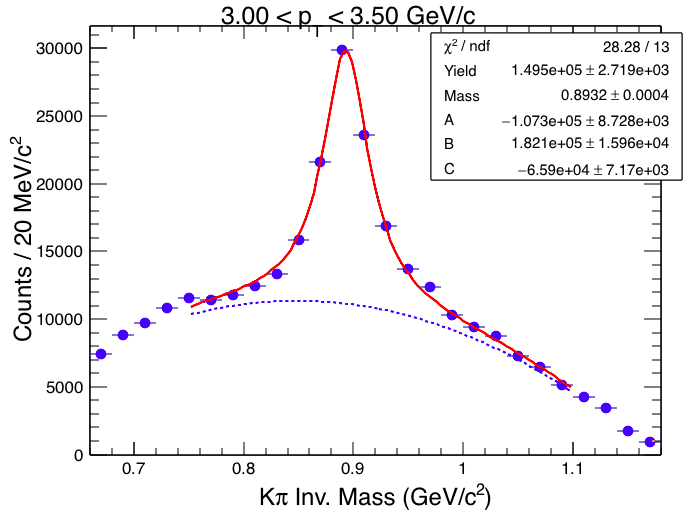
\includegraphics[width=2in]{Images/Chapter4/fit/7.png} &
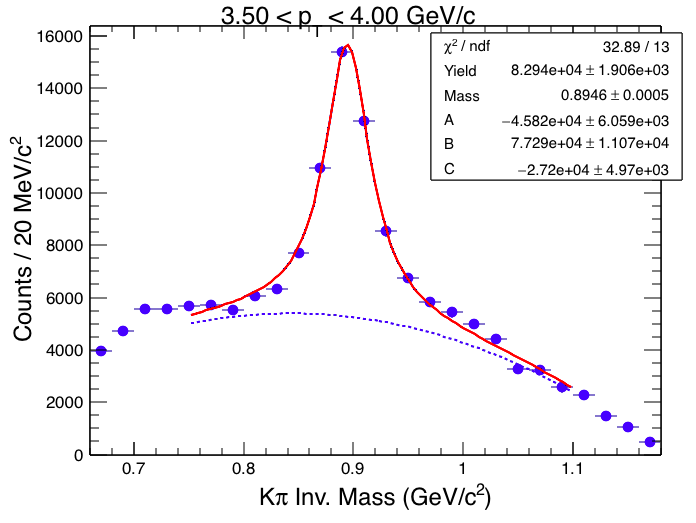
\includegraphics[width=2in]{Images/Chapter4/fit/8.png} \\
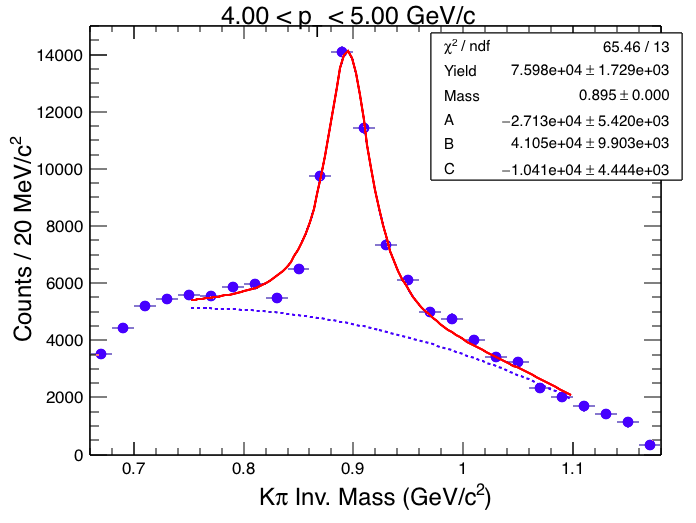
\includegraphics[width=2in]{Images/Chapter4/fit/9.png} &
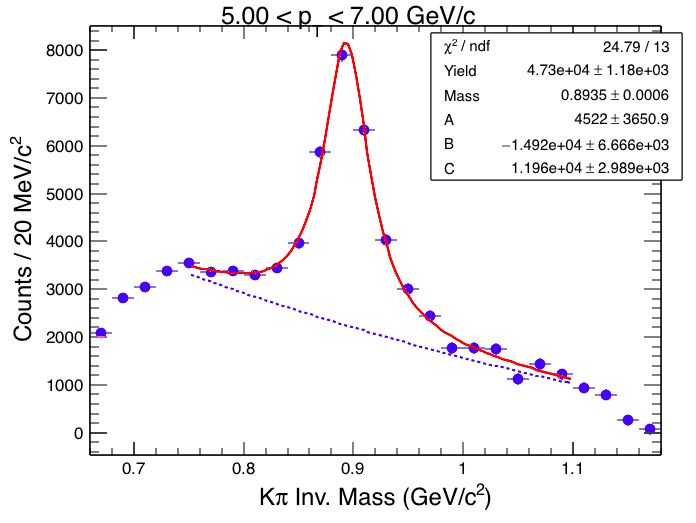
\includegraphics[width=2in]{Images/Chapter4/fit/10.png} &
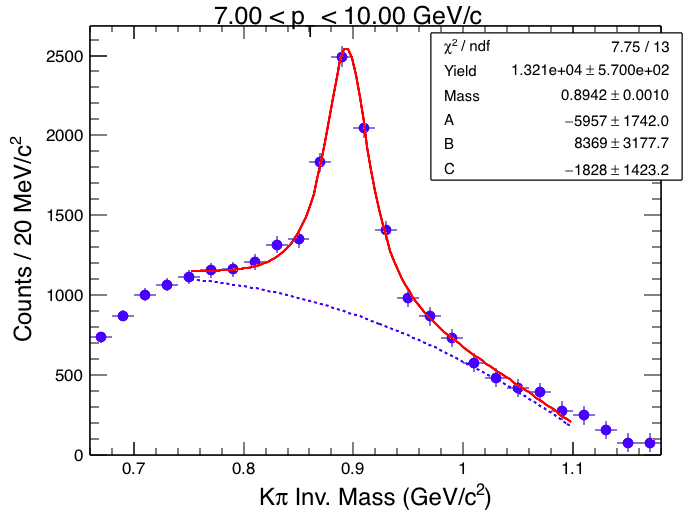
\includegraphics[width=2in]{Images/Chapter4/fit/11.png}
\end{array}$
\end{center}
\caption{Fitting results from different \pT~ regions for BW+ Polynomial function}
\label{Fig:chap4-4.6}
\end{figure}





\begin{figure}[H]
\begin{center}
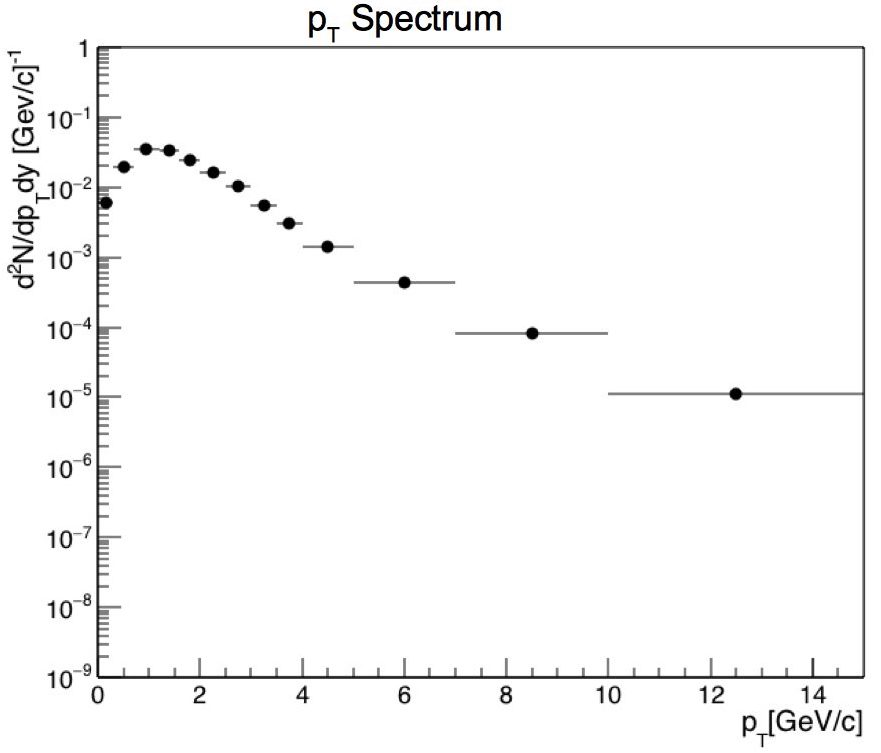
\includegraphics[width= 0.6\textwidth]{Images/Chapter4/k0ptspectra.jpg}
\caption{\kzero~ raw yield spectrum.}
\label{Fig:chap4-4.7}
\end{center}
\end{figure}



\section{Monte Carlo}
\label{par:4.6}
\subsection{Efficiency x acceptance of \kzero}
\label{par:4.6a}
Acceptance is defined as the percentage of generated particles whose final states are geometrically included in the detector. Efficiency takes into account detector limitations that for a given particle depend on the mass, charge, momentum etc. \\
\\
We use Monte Carlo productions to estimate our efficiency x acceptance. In our present case, we used the Monte Carlo production LHC15g3a3 which was generated using PYHTIA8 - Monash 2013. PYTHIA is an example of event generators which are software libraries that generate simulated high-energy particle physics events. In most processes a factorisation of the full process into individual problems is possible, these individual processes are calculated separately, and the probabilistic branching between them is performed using Monte Carlo methods. The final-state particles generated by event generator is fed into the detector simulation, allowing a precise prediction and verification for the entire system of experimental setup. 
\\
\\
The acceptance times efficiency is defined as the ratio of the number of reconstructed \kzero~ mesons having decay daughters ($K^{\pm}\pi^{\mp}$) that passes through the track cuts which are used in real data analysis to the number of generated \kzero~ with same decay daughter in rapidity interval $\pm 0.5$.

$$\epsilon_{rec}= \frac{N_{reconstructed}}{N_{generated}}$$
\\
The uncertainty in $\epsilon_{rec}$ is calculated using the Bayesian approach. The choice of bayesian approach is motivated by the fact that the events of numerator and denominator are correlated. The standard deviation for the efficiency $\epsilon_{rec} = k/n$, where the numerator $k$ is a subset of the denominator $n$, is:
$$\sigma_{\epsilon}= \sqrt{\frac{k+1}{n+2} \left( \frac{k+2}{n+3}- \frac{k+1}{n+2}\right)}$$

The \kzero~ acceptance x efficiency distribution as a function of \pT~ is shown in \mbox{Figure \ref{Fig:chap4-4.8}}. 

\begin{figure}[H]
\begin{center}
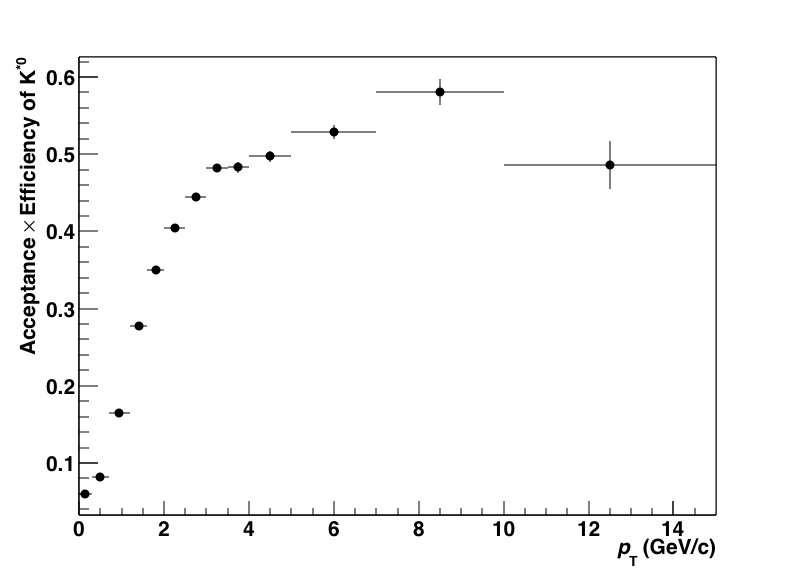
\includegraphics[width= 0.6\textwidth]{Images/Chapter4/effre.png}
\caption{Efficiency x Acceptance vs \pT~ for \kzero~ }
\label{Fig:chap4-4.8}
\end{center}
\end{figure}


\subsection{Corrected \pT~ spectrum}
\label{par:4.6b}
To extract the yield, raw counts were corrected for the decay branching ratio(BR), and for the losses due to pion/kaon in-flight decays, geometrical acceptance and detector efficiency(eff) ($N_{cor}= \text{Raw Counts}/  \text{BR x eff}$). Absolute resonance yield in inelastic collisions is estimated using the following formula:

$$\frac{d^{2}N}{dp_{T}dy} = \frac{\text{Raw Counts}}{N_{MB} \times BR \times dp_{T} \times dy \times eff} \times f_{norm} \times f_{SL}$$

where $N_{MB}$ is the number of the minimum bias trigger selected by the event cuts, BR is the branching ratio (which is the fraction of particles decaying in the desired decay mode with respect to the total number of particles decaying), $eff$ is the acceptance x efficiency of reconstruction. The factor $f_{norm}= 0.852^{+0.062}_{-0.03}$ is efficiency for trigger selection for inelastic pp collisions.  The factor $f_{SL} = 0.931264$ accounts for the signal loss introduced by the requirement that a primary vertex must be reconstructed and be in the range of  $\pm 10$ cm.
\\
\\
The correct value for $f_{norm}$ for Run2 data is not yet accurately known so we use the value from Run1. 
\\
\\
The obtained \pT~ spectrum for \kzero~ is shown in \mbox{Figure \ref{Fig:chap4-4.9}}. 

\begin{figure}[H]
\begin{center}
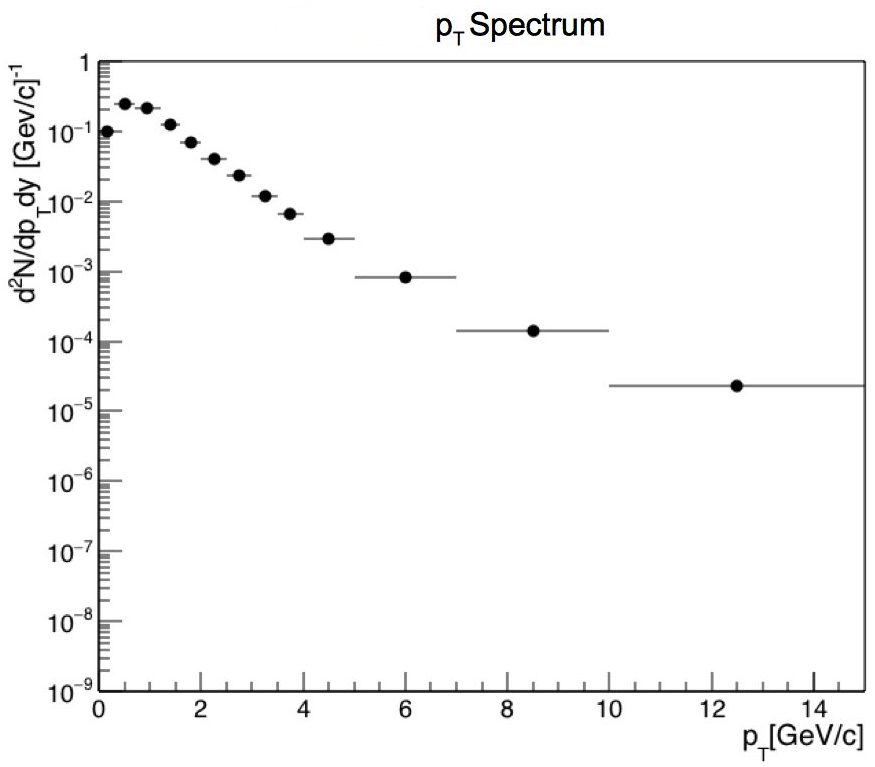
\includegraphics[width= 0.8\textwidth]{Images/Chapter4/k0corrected.png}
\caption{Transverse momentum spectrum of \kzero~ produced in pp collisions at $\sqrt{s}= 13$ TeV }
\label{Fig:chap4-4.9}
\end{center}
\end{figure}



\begin{figure}[H]
\begin{center}
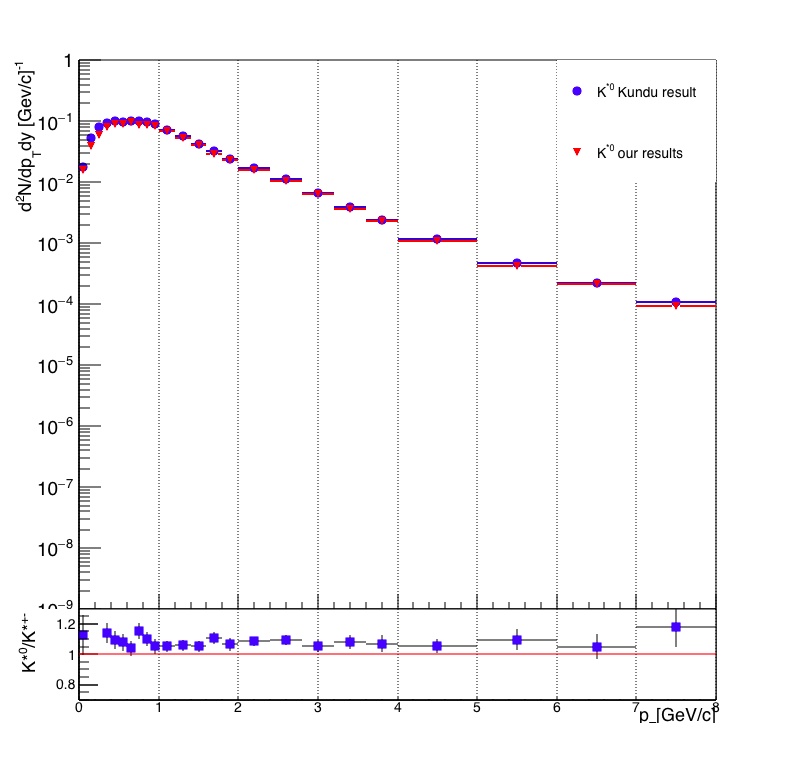
\includegraphics[width= 0.6\textwidth]{Images/Chapter4/compkish.png}
\caption{Spectra comparison with approved results.}
\label{Fig:chap4-4.10}
\end{center}
\end{figure}


\mbox{Figure \ref{Fig:chap4-4.10}}.  is the comparison between the official \pT spectrum (blue symbols) and the ones obtained in this analysis (red symbols) . The results are divided by a factor of 2 to account for \kzero~  $+ \overline{K}^{*0}$ and corrected for branching ratio and efficiency only.















